\documentclass[11pt,letterpaper]{article}
\usepackage[margin=1in]{geometry}
\usepackage{graphicx}
\usepackage{hyperref}
\usepackage{enumitem}
\usepackage{amsmath}
\usepackage{amsfonts}
\usepackage{booktabs}
\usepackage{xcolor}
\usepackage{fancyhdr}
\usepackage{titlesec}
\usepackage{url}
\usepackage{float}

% Configure hyperlinks
\hypersetup{
    colorlinks=true,
    linkcolor=blue,
    urlcolor=blue,
    citecolor=blue
}

% Configure headers
\pagestyle{fancy}
\fancyhf{}
\rhead{Jiang | Immigrants Against Immigrants?}
\lhead{ASA 2025}
\cfoot{\thepage}

% Configure section formatting
\titleformat{\section}{\Large\bfseries}{\thesection}{1em}{}
\titleformat{\subsection}{\large\bfseries}{\thesubsection}{1em}{}
\titleformat{\subsubsection}{\normalsize\bfseries}{\thesubsubsection}{1em}{}

% Configure list formatting
\setlist[itemize,1]{leftmargin=1em,label=\textbullet}
\setlist[itemize,2]{leftmargin=1.5em,label=$\circ$}
\setlist[itemize,3]{leftmargin=2em,label=$-$}
\setlist[enumerate,1]{leftmargin=1em}

\title{\textbf{Immigrants Against Immigrants?}\\
\large Mapping Generational Trends in Anti-Immigration Attitudes among U.S. Hispanics, 2002--2023}

\author{Ann Jiang, UC San Diego\\
\href{mailto:annjiang@ucsd.edu}{annjiang@ucsd.edu} | \href{https://github.com/annjiangcodes}{github.com/annjiangcodes}}

\date{}

\begin{document}

\maketitle

\section{Central Puzzle \& Research Questions}

\subsection{Motivation}
\begin{itemize}
    \item \textbf{Media narratives}: Growing Hispanic support for restrictionist candidates
    \item \textbf{Electoral data}: Latino Trump vote share increased 2016$\rightarrow$2020
    \item \textbf{Theoretical puzzle}: Why would immigrants support anti-immigration policies?
\end{itemize}

\textbf{Puzzle:} Why do some Hispanic immigrants, who have benefited from immigration, support restrictionist immigration policies? This contradicts simple group solidarity theories and aligns with growing media narratives of a conservative shift.

\subsection{Core Questions}
\begin{enumerate}
    \item \textbf{Prevalence:} How common are restrictionist views among U.S. Hispanics?
    \item \textbf{Trends:} How have these attitudes changed over the last 20 years?
    \item \textbf{Generations:} How do attitudes differ between 1st, 2nd, and 3rd+ generation Hispanics?
    \item \textbf{Mechanisms:} What explains these differences?
\end{enumerate}

\section{Data \& Methodology}

\subsection{Data Source}

\textbf{Pew Research Center's National Survey of Latinos (NSL)}
\begin{itemize}
    \item \textbf{Scope:} 14 survey waves from 2002--2023
    \item \textbf{Sample:} 37,496 respondents across 21 years
    \item \textbf{Coverage:} 4 presidential administrations (Bush, Obama, Trump, Biden)
\end{itemize}

\subsection{Analytical Approach}
\begin{itemize}
    \item Generation-stratified models
    \item Linear regression with year as continuous
    \item Survey-weighted representative estimates
    \item Complete case analysis: 16,327 cases (43.5\% of total sample)
\end{itemize}

\subsection{Key Methodological Innovation: Moving Beyond a Single ``Pro/Anti'' Scale}

\textbf{Initial Problem:} Single-index approach masked crucial differences in attitudes.

\textbf{Solution:} Three distinct indices constructed to capture attitude complexity:

\begin{enumerate}
    \item \textbf{Immigration Policy Liberalism}
    \begin{itemize}
        \item Components: Support for legalization, DACA support
        \item Coverage: 8+ years, 61\% of observations
        \item Interpretation: Higher = more liberal immigration policies
    \end{itemize}
    
    \item \textbf{Immigration Policy Restrictionism}
    \begin{itemize}
        \item Components: Border wall support, deportation policy support, ``too many immigrants''
        \item Coverage: 9+ years, 64\% of observations
        \item Interpretation: Higher = more restrictionist immigration policies
    \end{itemize}
    
    \item \textbf{Deportation Concern}
    \begin{itemize}
        \item Components: Personal deportation worry
        \item Coverage: 4+ years, 22\% of observations
        \item Interpretation: Higher = greater deportation concerns
    \end{itemize}
\end{enumerate}

\begin{figure}[H]
    \centering
    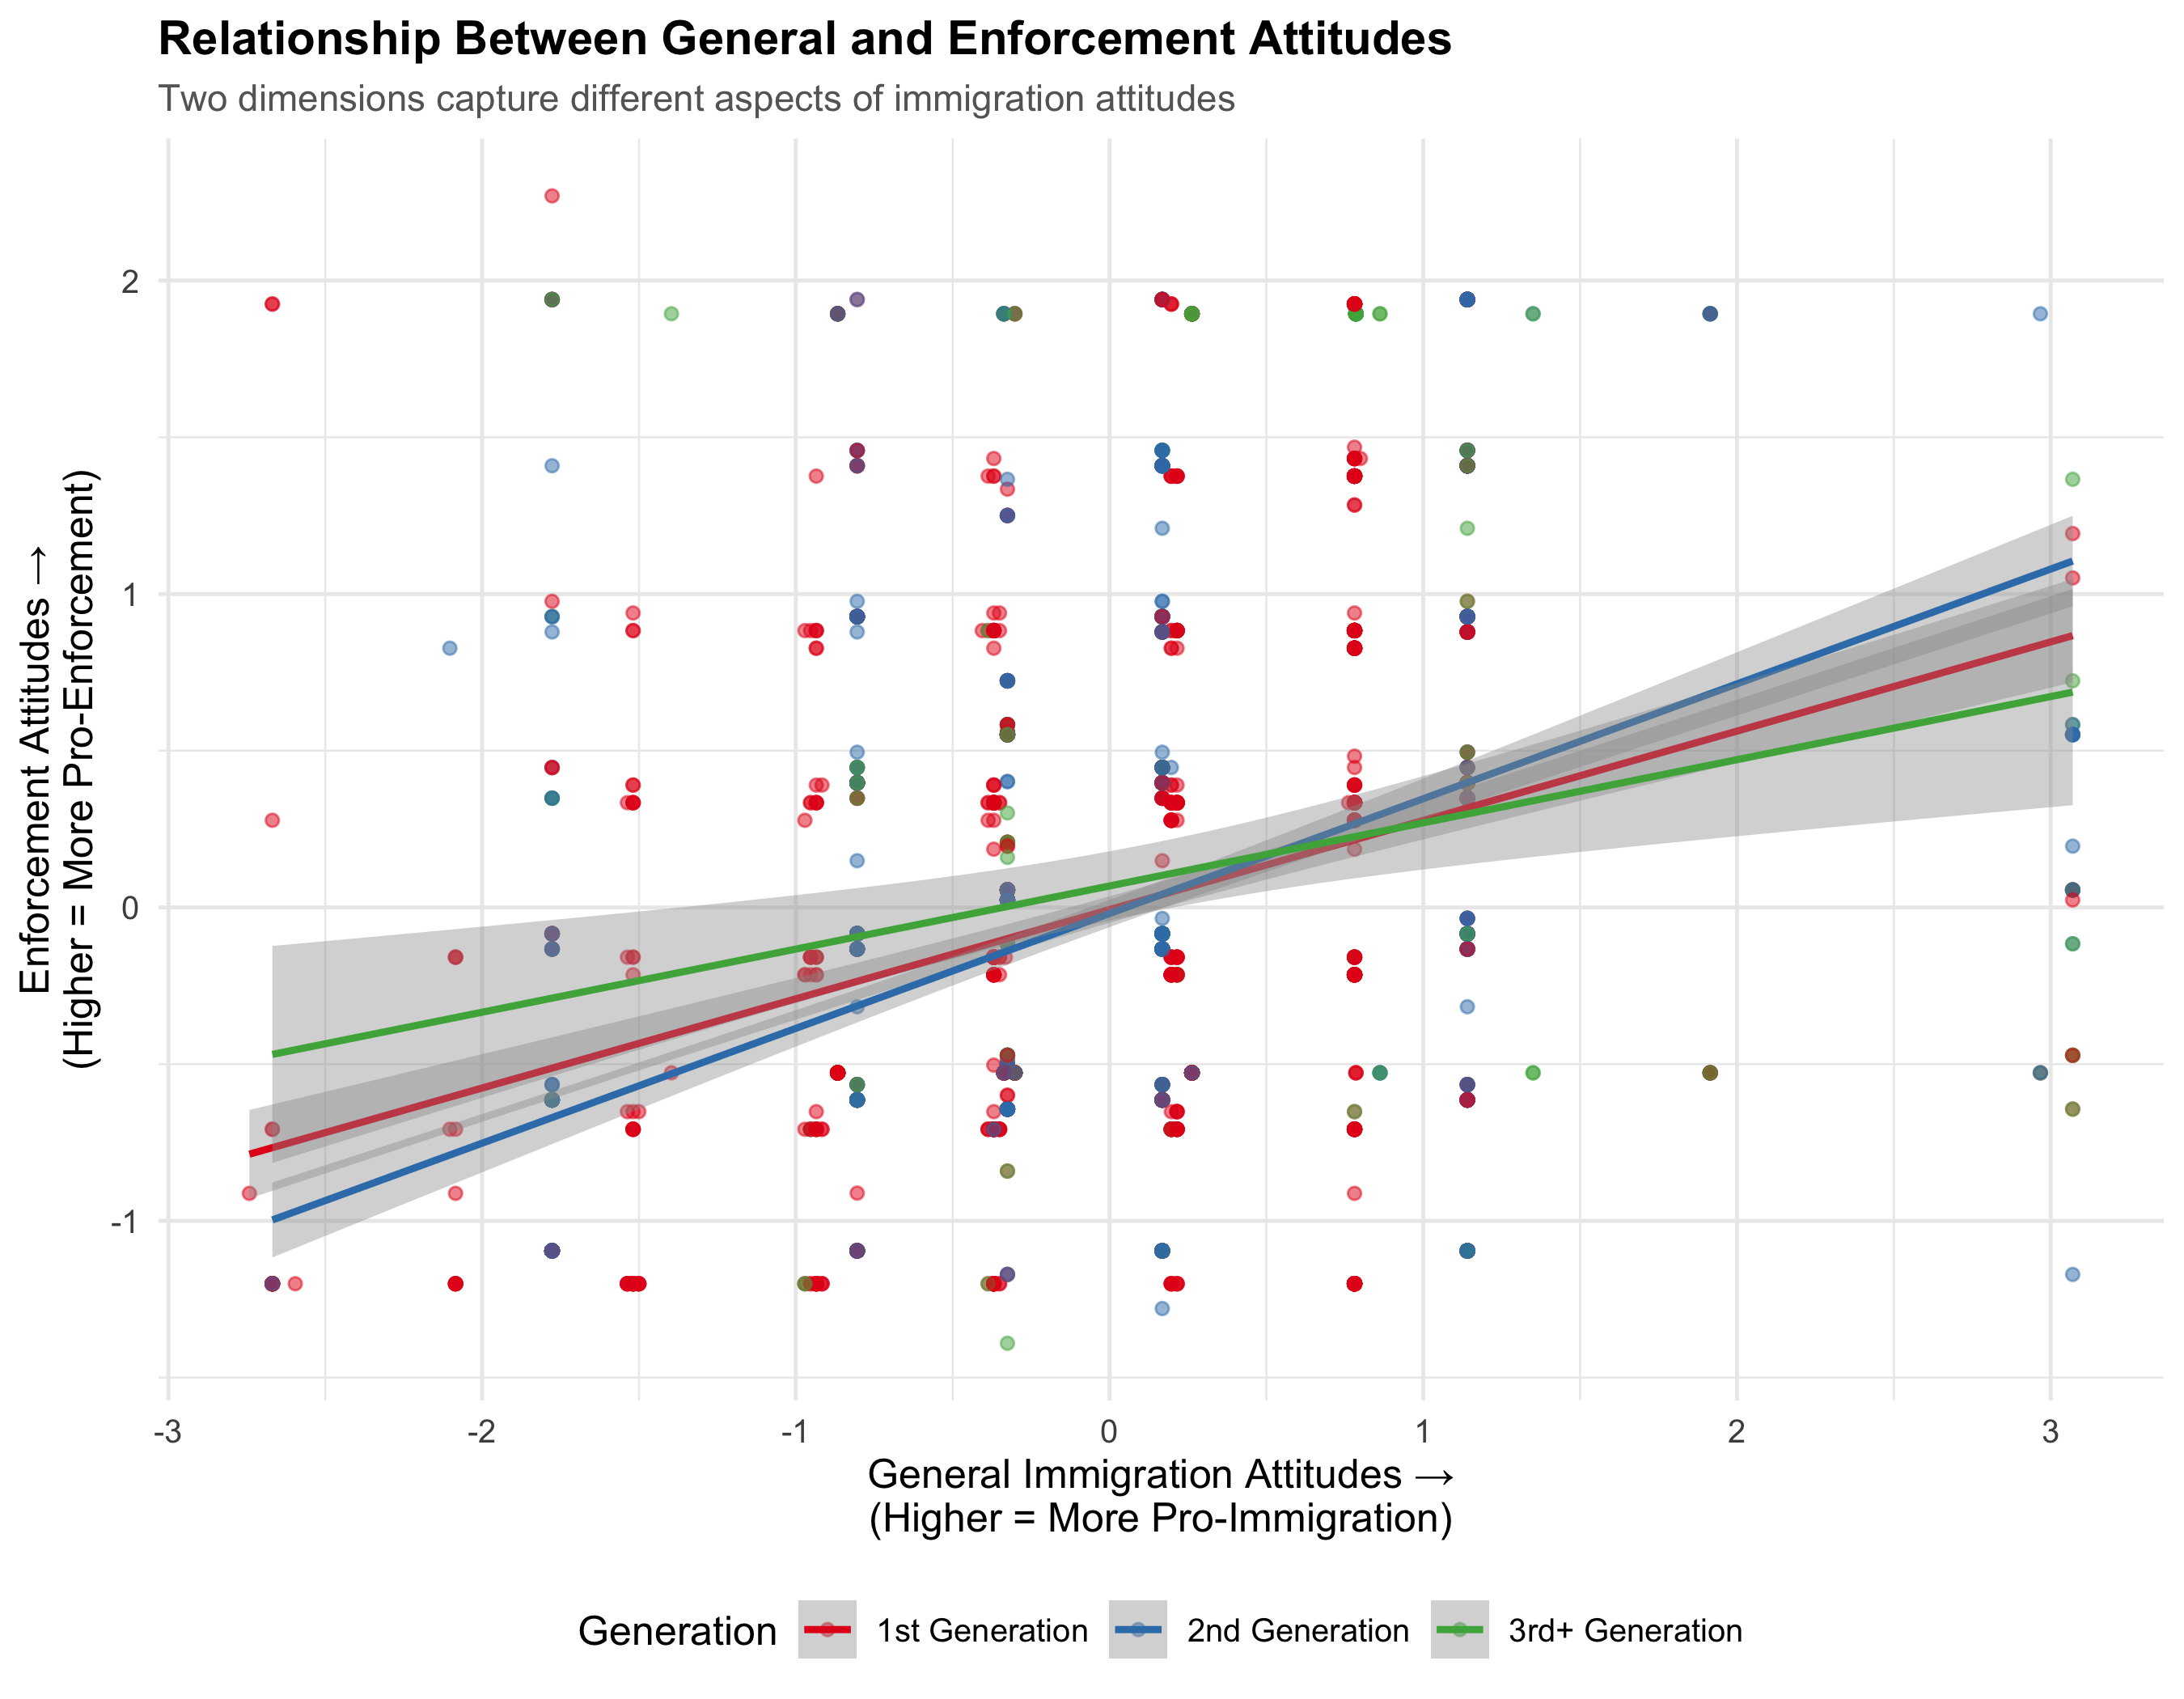
\includegraphics[width=0.8\textwidth]{figure_v4_2_dimensions_scatter_robust.png}
    \caption{Two dimensions capture different aspects of immigration attitudes}
    \label{fig:dimensions}
\end{figure}

\subsection{Generational Coding}
\begin{itemize}
    \item \textbf{1st Gen:} Foreign-born
    \item \textbf{2nd Gen:} U.S.-born, at least one foreign-born parent
    \item \textbf{3rd+ Gen:} U.S.-born, U.S.-born parents
\end{itemize}

\section{Key Findings}

\subsection{The Illusion of Stability}

Across the total Hispanic population, aggregate attitudes on immigration appear \textbf{remarkably stable} over 20 years. However, \textbf{this stability masks significant and diverging trends between immigrant generations.}

\subsection{Generational Divergence (The Core Finding)}

\textbf{Statistical Evidence (Survey-Weighted v2.8)}

\textbf{First Generation:}
\begin{itemize}
    \item \textbf{Liberalism:} +0.019 per year (p=0.021*)
    \item \textbf{Restrictionism:} +0.011 per year (p=0.004**)
    \item \textbf{Pattern:} Becoming simultaneously \textbf{more liberal AND more restrictionist}
    \item Support for legalization is increasing, but so is support for enforcement
\end{itemize}

\textbf{Second Generation:}
\begin{itemize}
    \item \textbf{Liberalism:} -0.005 per year (p=0.488, ns)
    \item \textbf{Restrictionism:} -0.015 per year (p=0.056, ns)
    \item \textbf{Pattern:} Attitudes \textbf{converging toward the middle}, with decreasing extremity on both sides
\end{itemize}

\textbf{Third+ Generation:}
\begin{itemize}
    \item \textbf{Liberalism:} -0.016 per year (p=0.158, ns)
    \item \textbf{Restrictionism:} -0.002 per year (p=0.908, ns)
    \item \textbf{Pattern:} Remain the \textbf{most consistently restrictionist} group, with stable attitudes over time
\end{itemize}

\begin{figure}[H]
    \centering
    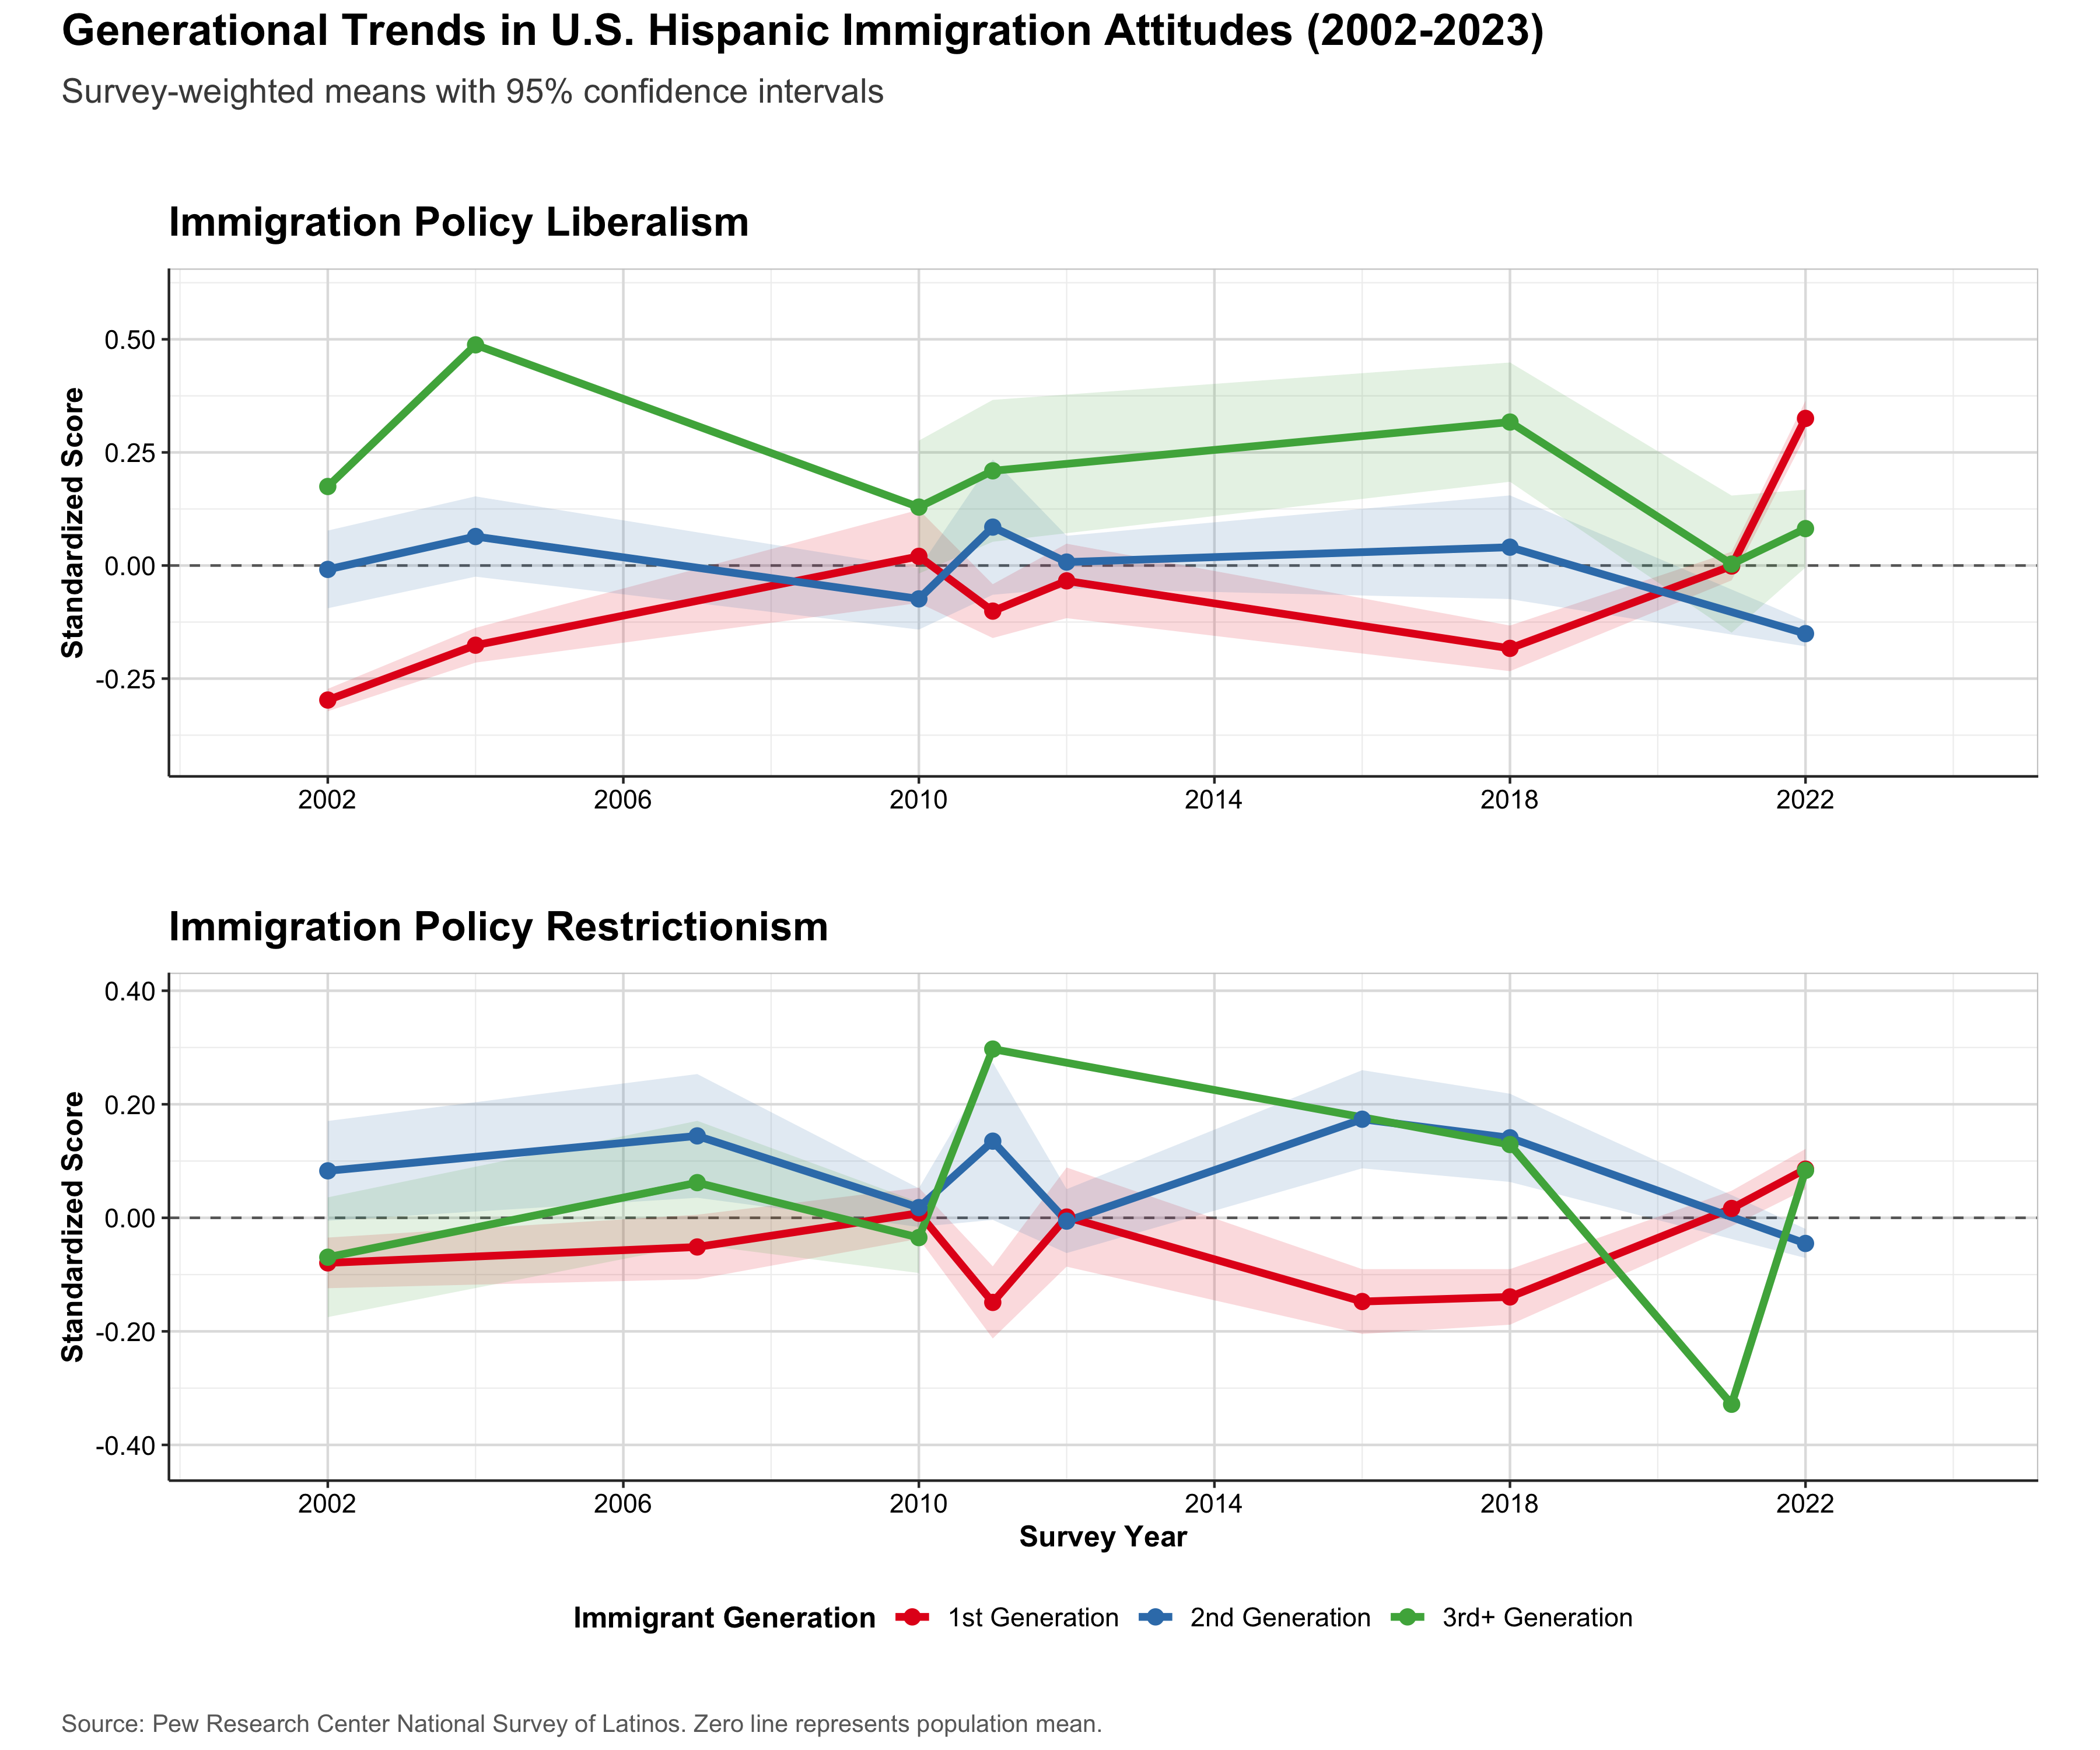
\includegraphics[width=0.9\textwidth]{figure_v4_4_main_generation_trends.png}
    \caption{Generational Trends in U.S. Hispanic Immigration Attitudes (2002-2023)}
    \label{fig:main_trends}
\end{figure}

\begin{figure}[H]
    \centering
    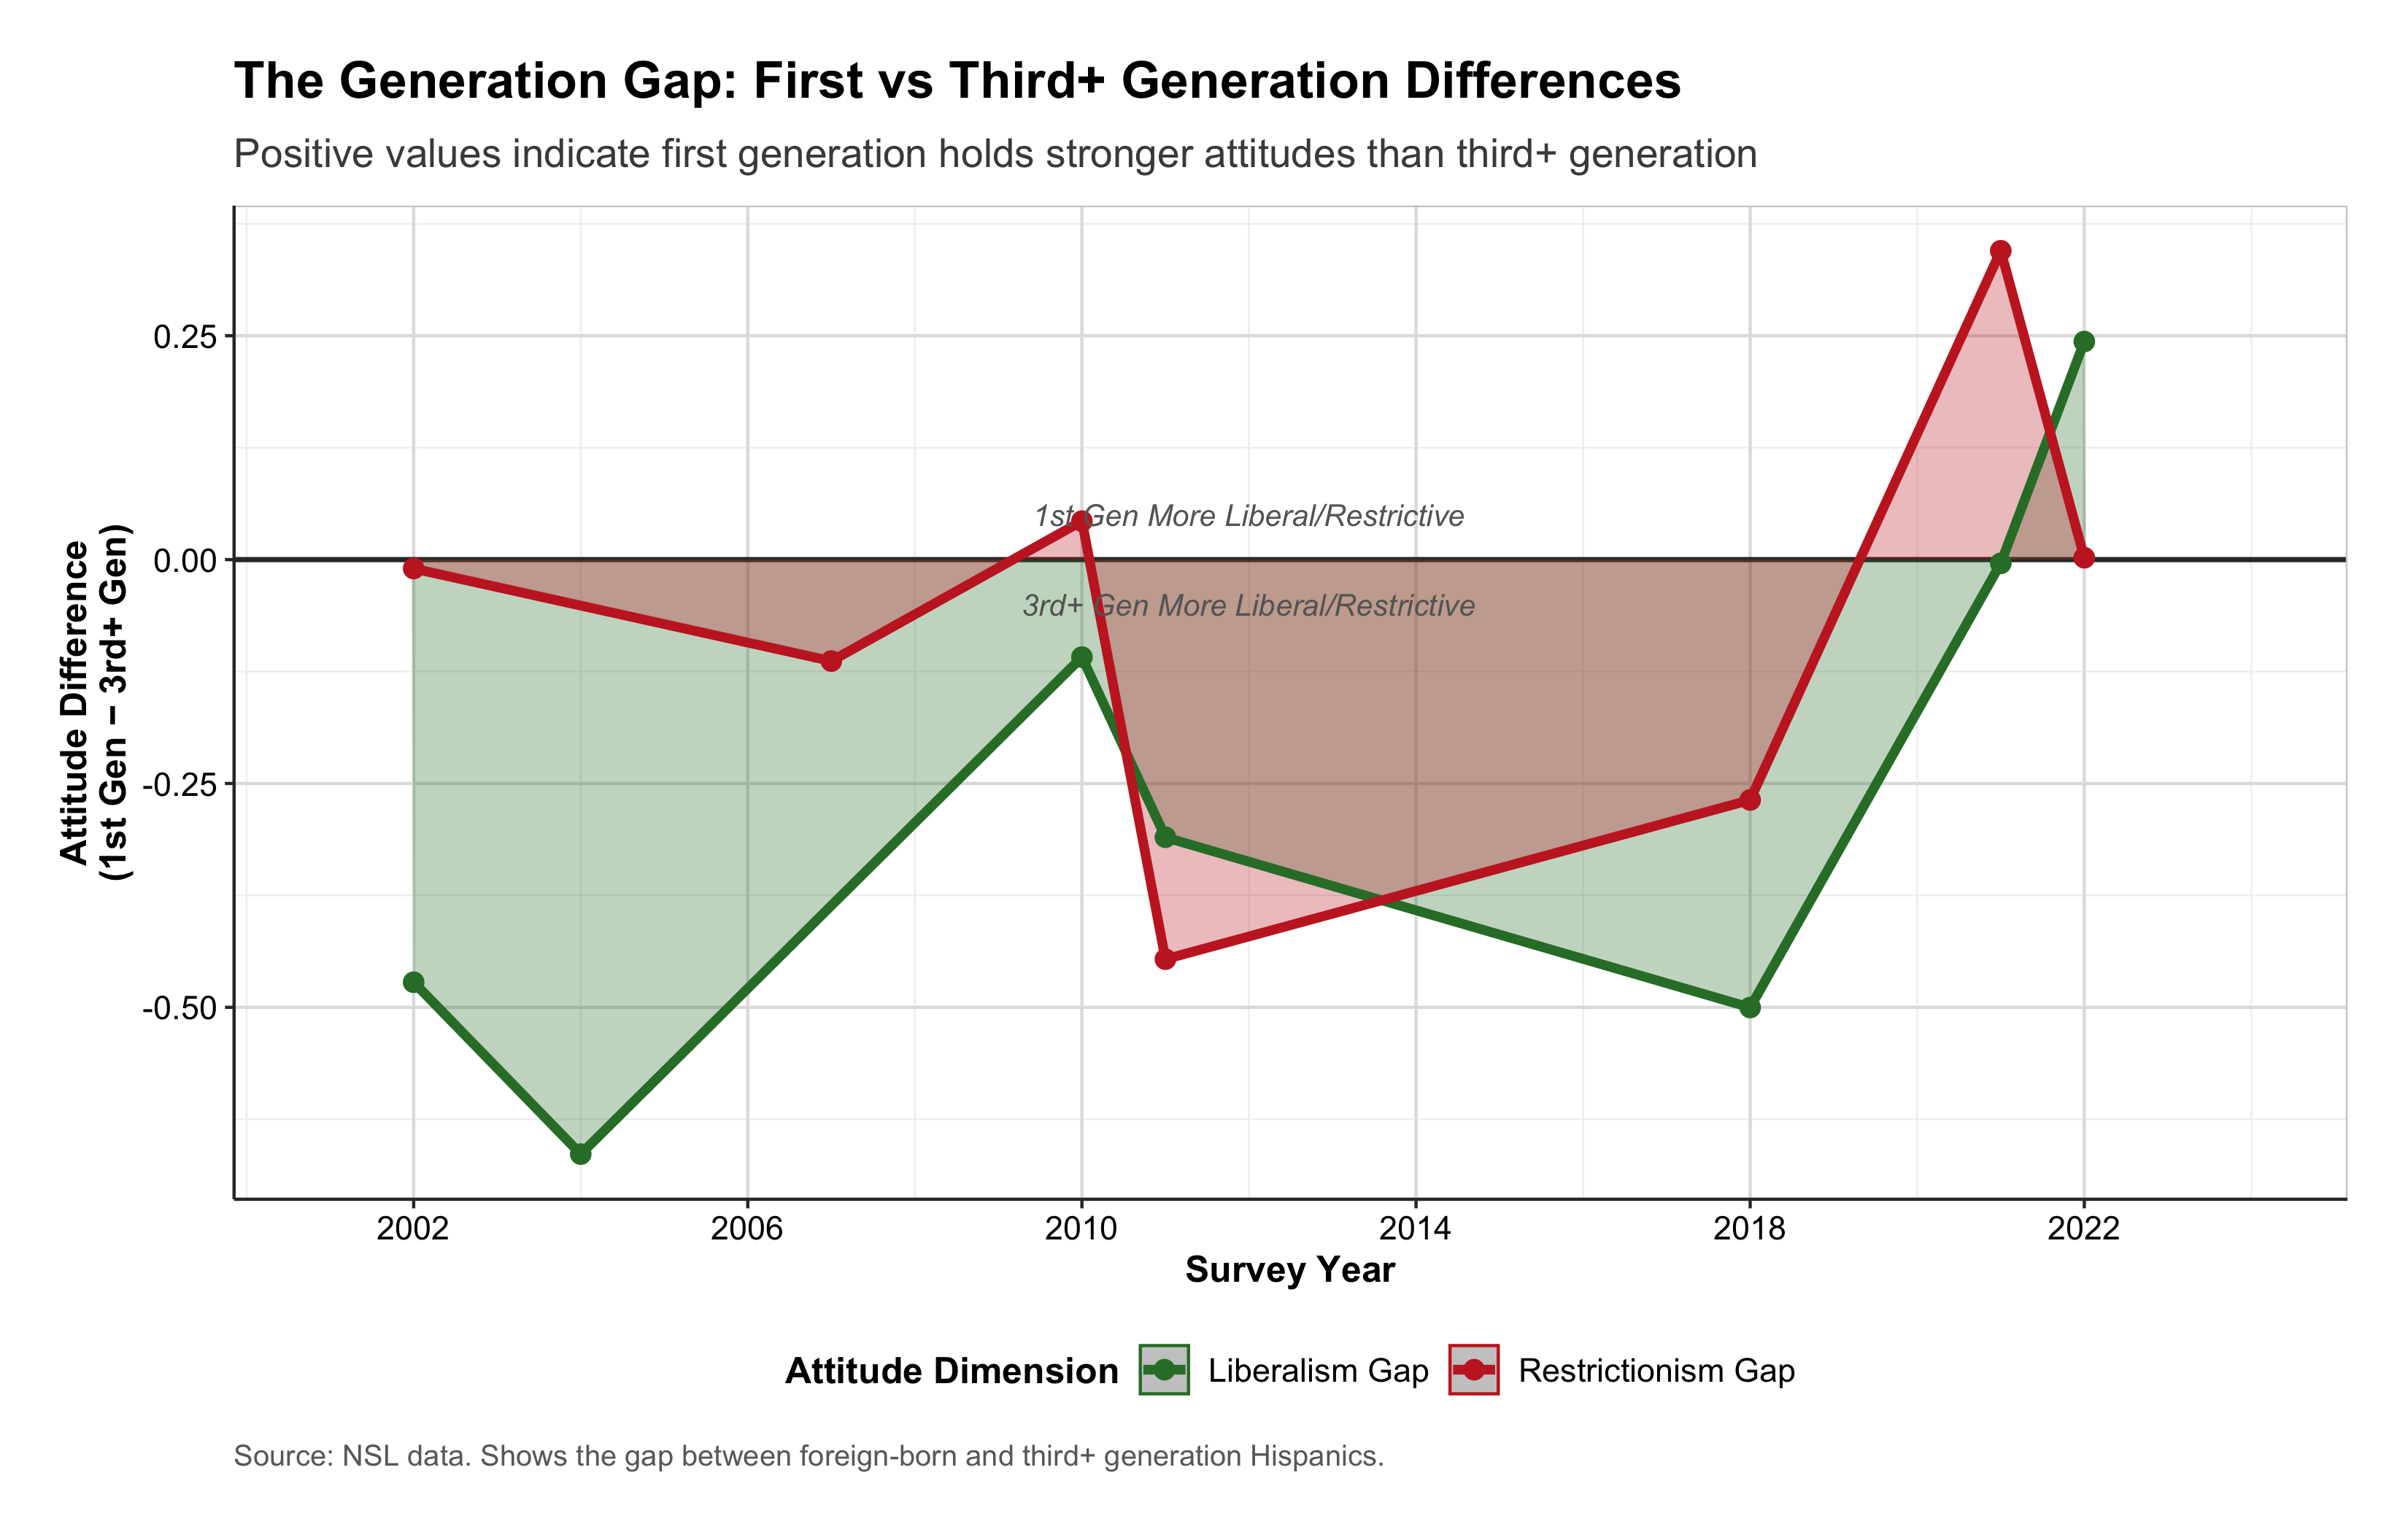
\includegraphics[width=0.9\textwidth]{figure_v4_4_generation_gap.png}
    \caption{The Generation Gap: First vs Third+ Generation Differences}
    \label{fig:generation_gap}
\end{figure}

\subsection{The ``Border Wall Paradox'' (Discovered via Disaggregated Analysis)}

Looking at individual policy components reveals dynamics hidden by aggregate indices. The most striking example is support for a border wall:

\textbf{Border Wall Support:}
\begin{itemize}
    \item \textbf{1st Generation:} Support for the wall has \textbf{decreased} over time
    \item \textbf{2nd Generation:} Support for the wall has \textbf{increased} over time
    \item \textbf{3rd+ Generation:} Support remains \textbf{stably high}
\end{itemize}

\textbf{Interpretation:} This finding directly contradicts linear assimilation theories.

\subsubsection{Heterogeneity Within Indices}
\begin{itemize}
    \item Variables within same index don't always correlate
    \item \textbf{Example:} Border wall negatively correlates with border security (r=-0.44)
    \item \textbf{Suggests:} Attitudes are fragmented
    \item \textbf{Immigration attitudes contain distinct modules:}
    \begin{itemize}
        \item Humanitarian concerns (DACA, legalization)
        \item Security/enforcement preferences
        \item Personal threat perception
        \item Economic competition beliefs?
    \end{itemize}
\end{itemize}

\subsubsection{Fragmentation Pattern}
\begin{itemize}
    \item Can support legalization AND enforcement
    \item Can oppose border wall but support deportation
    \item Personal concern $\neq$ policy preferences
\end{itemize}

\begin{figure}[H]
    \centering
    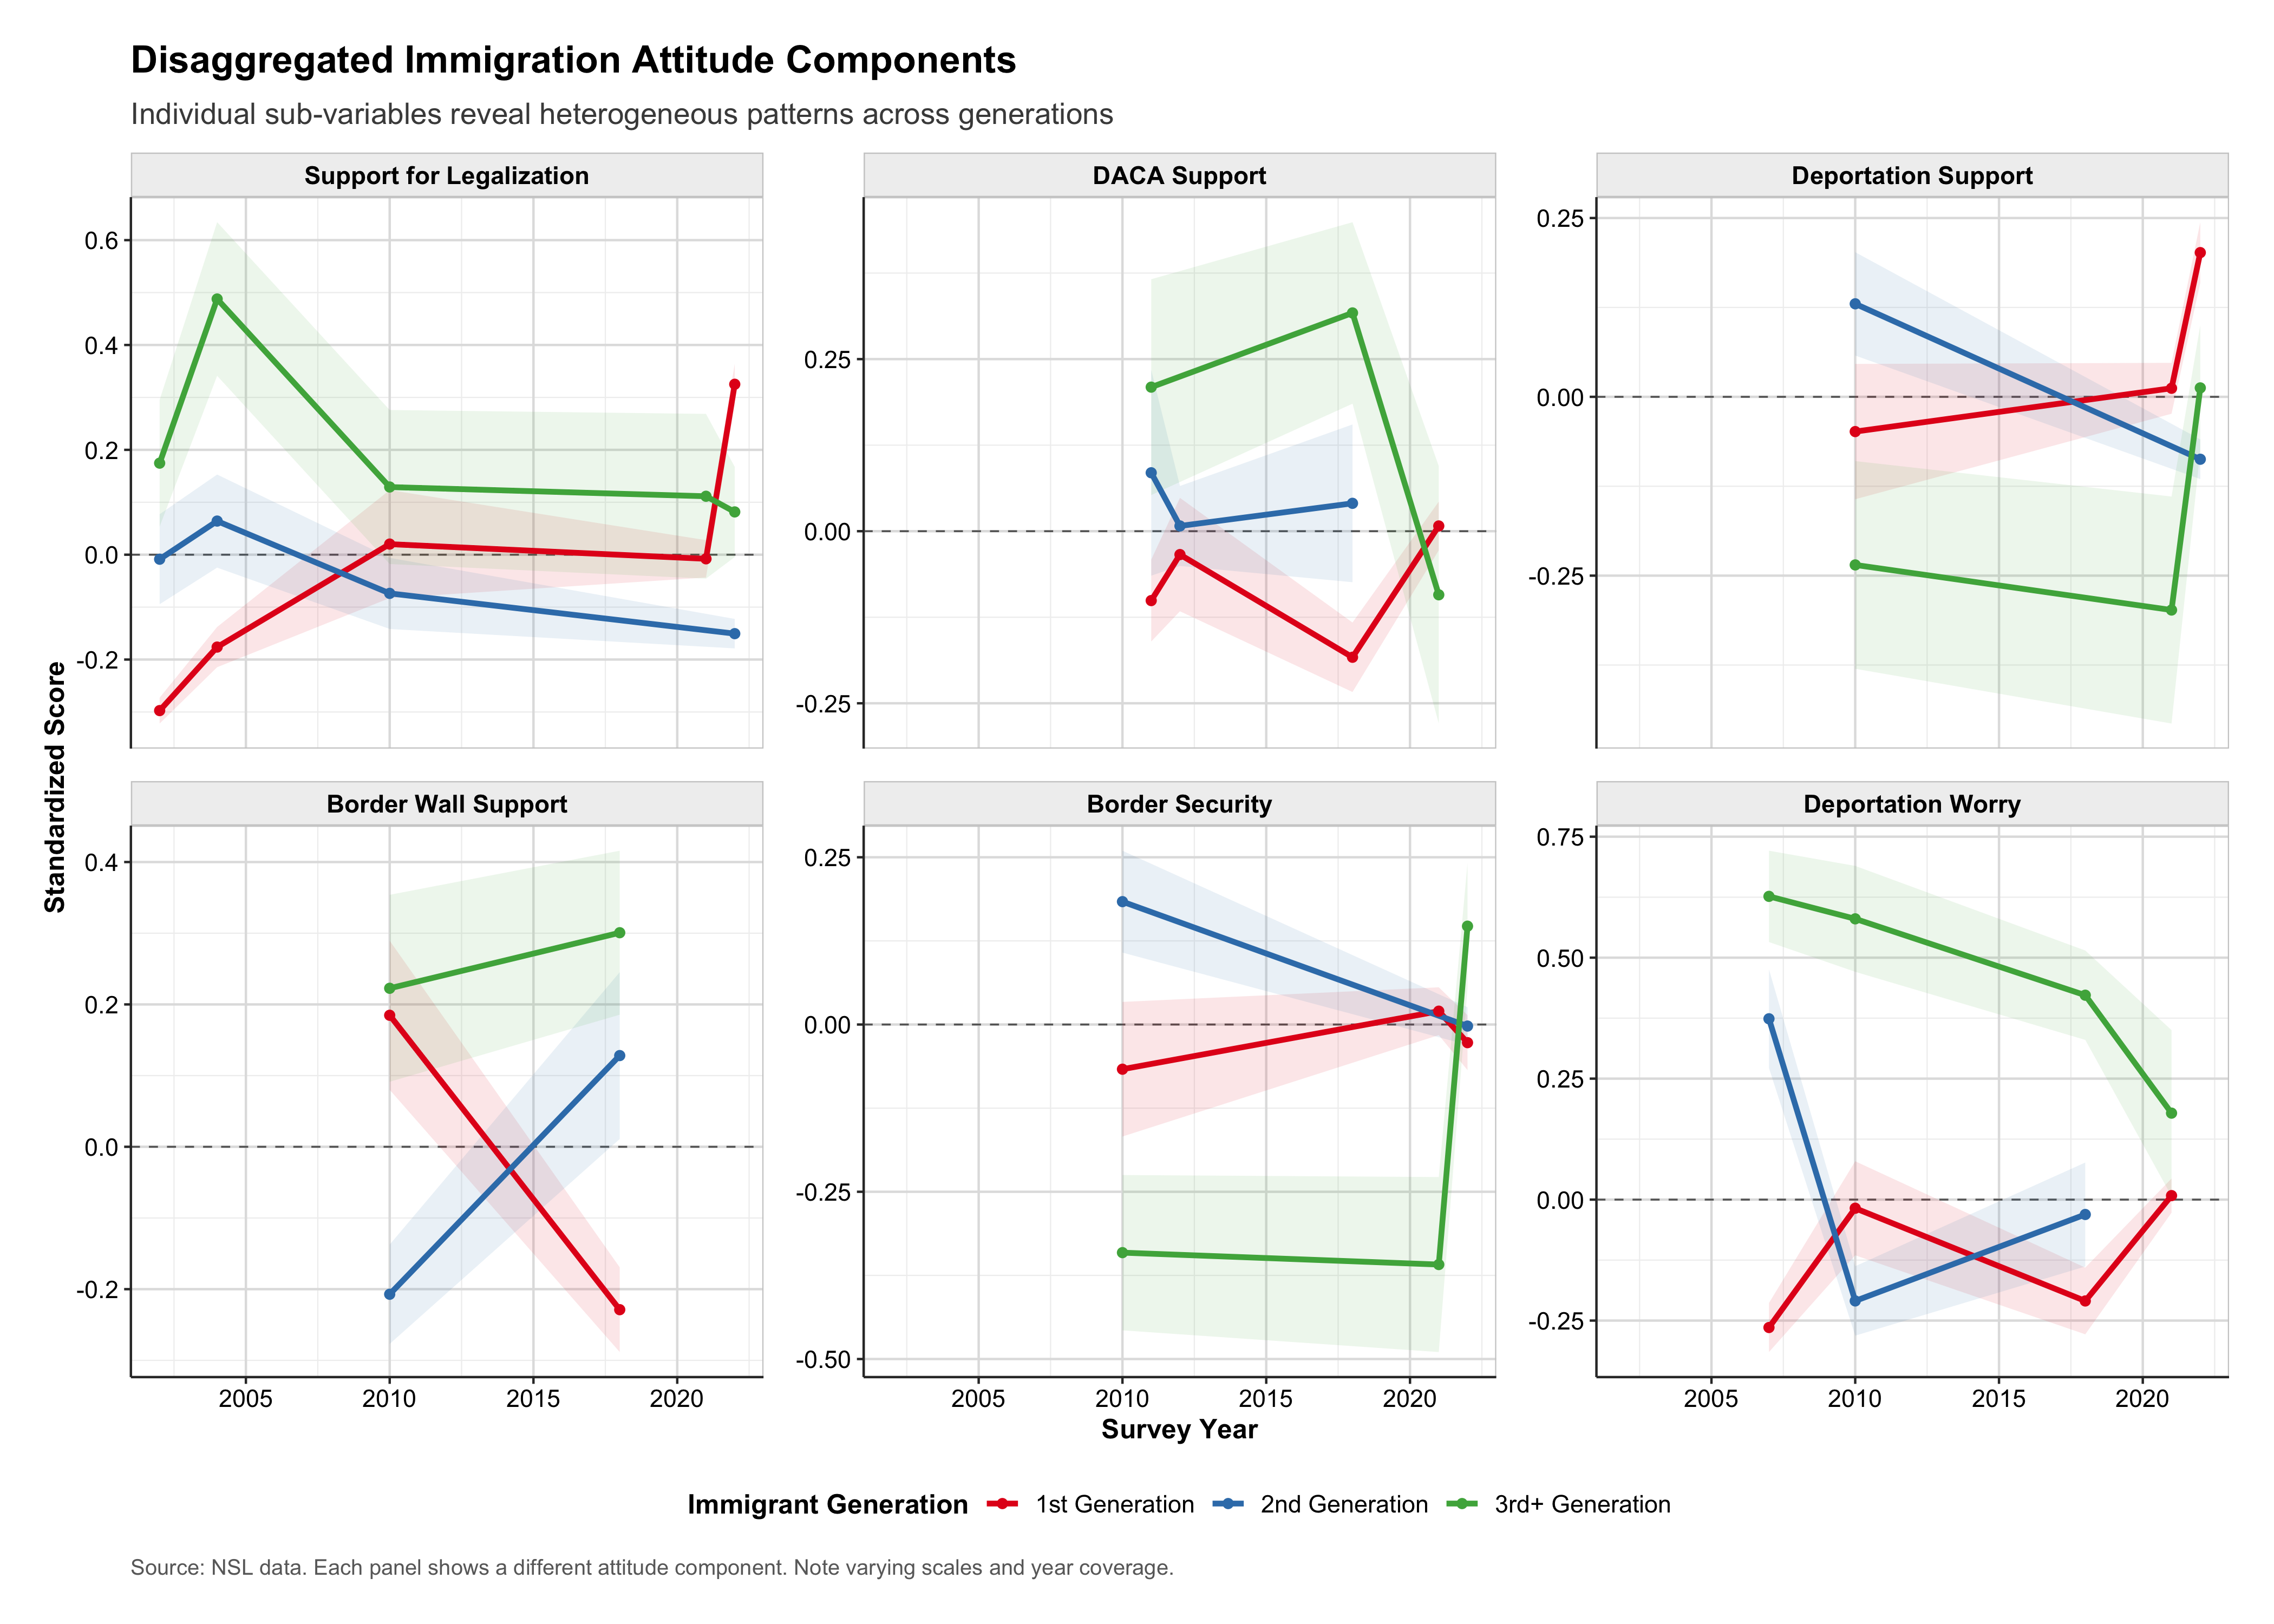
\includegraphics[width=0.9\textwidth]{figure_v4_4_disaggregated_components.png}
    \caption{Disaggregated Immigration Attitude Components}
    \label{fig:disaggregated}
\end{figure}

\subsection{The Power of Context: Period Effects}

Attitudes are shaped by political moments:
\begin{itemize}
    \item \textbf{Trump Era (2016-18):} Triggered ``defensive liberalization'' among 1st generation immigrants
    \item \textbf{Economic Crisis (2008-10):} All generations became temporarily more restrictionist
    \item \textbf{Obama Era:} Peak liberalism for 1st/2nd generation
\end{itemize}

\textbf{Key Period $\times$ Generation Interactions:}
\begin{itemize}
    \item \textbf{Trump Era:} 1st generation defensive liberalization
    \item \textbf{Economic Crisis:} All generations more restrictive
    \item \textbf{Obama Era:} Peak liberalism for 1st/2nd generation
\end{itemize}

\begin{figure}[H]
    \centering
    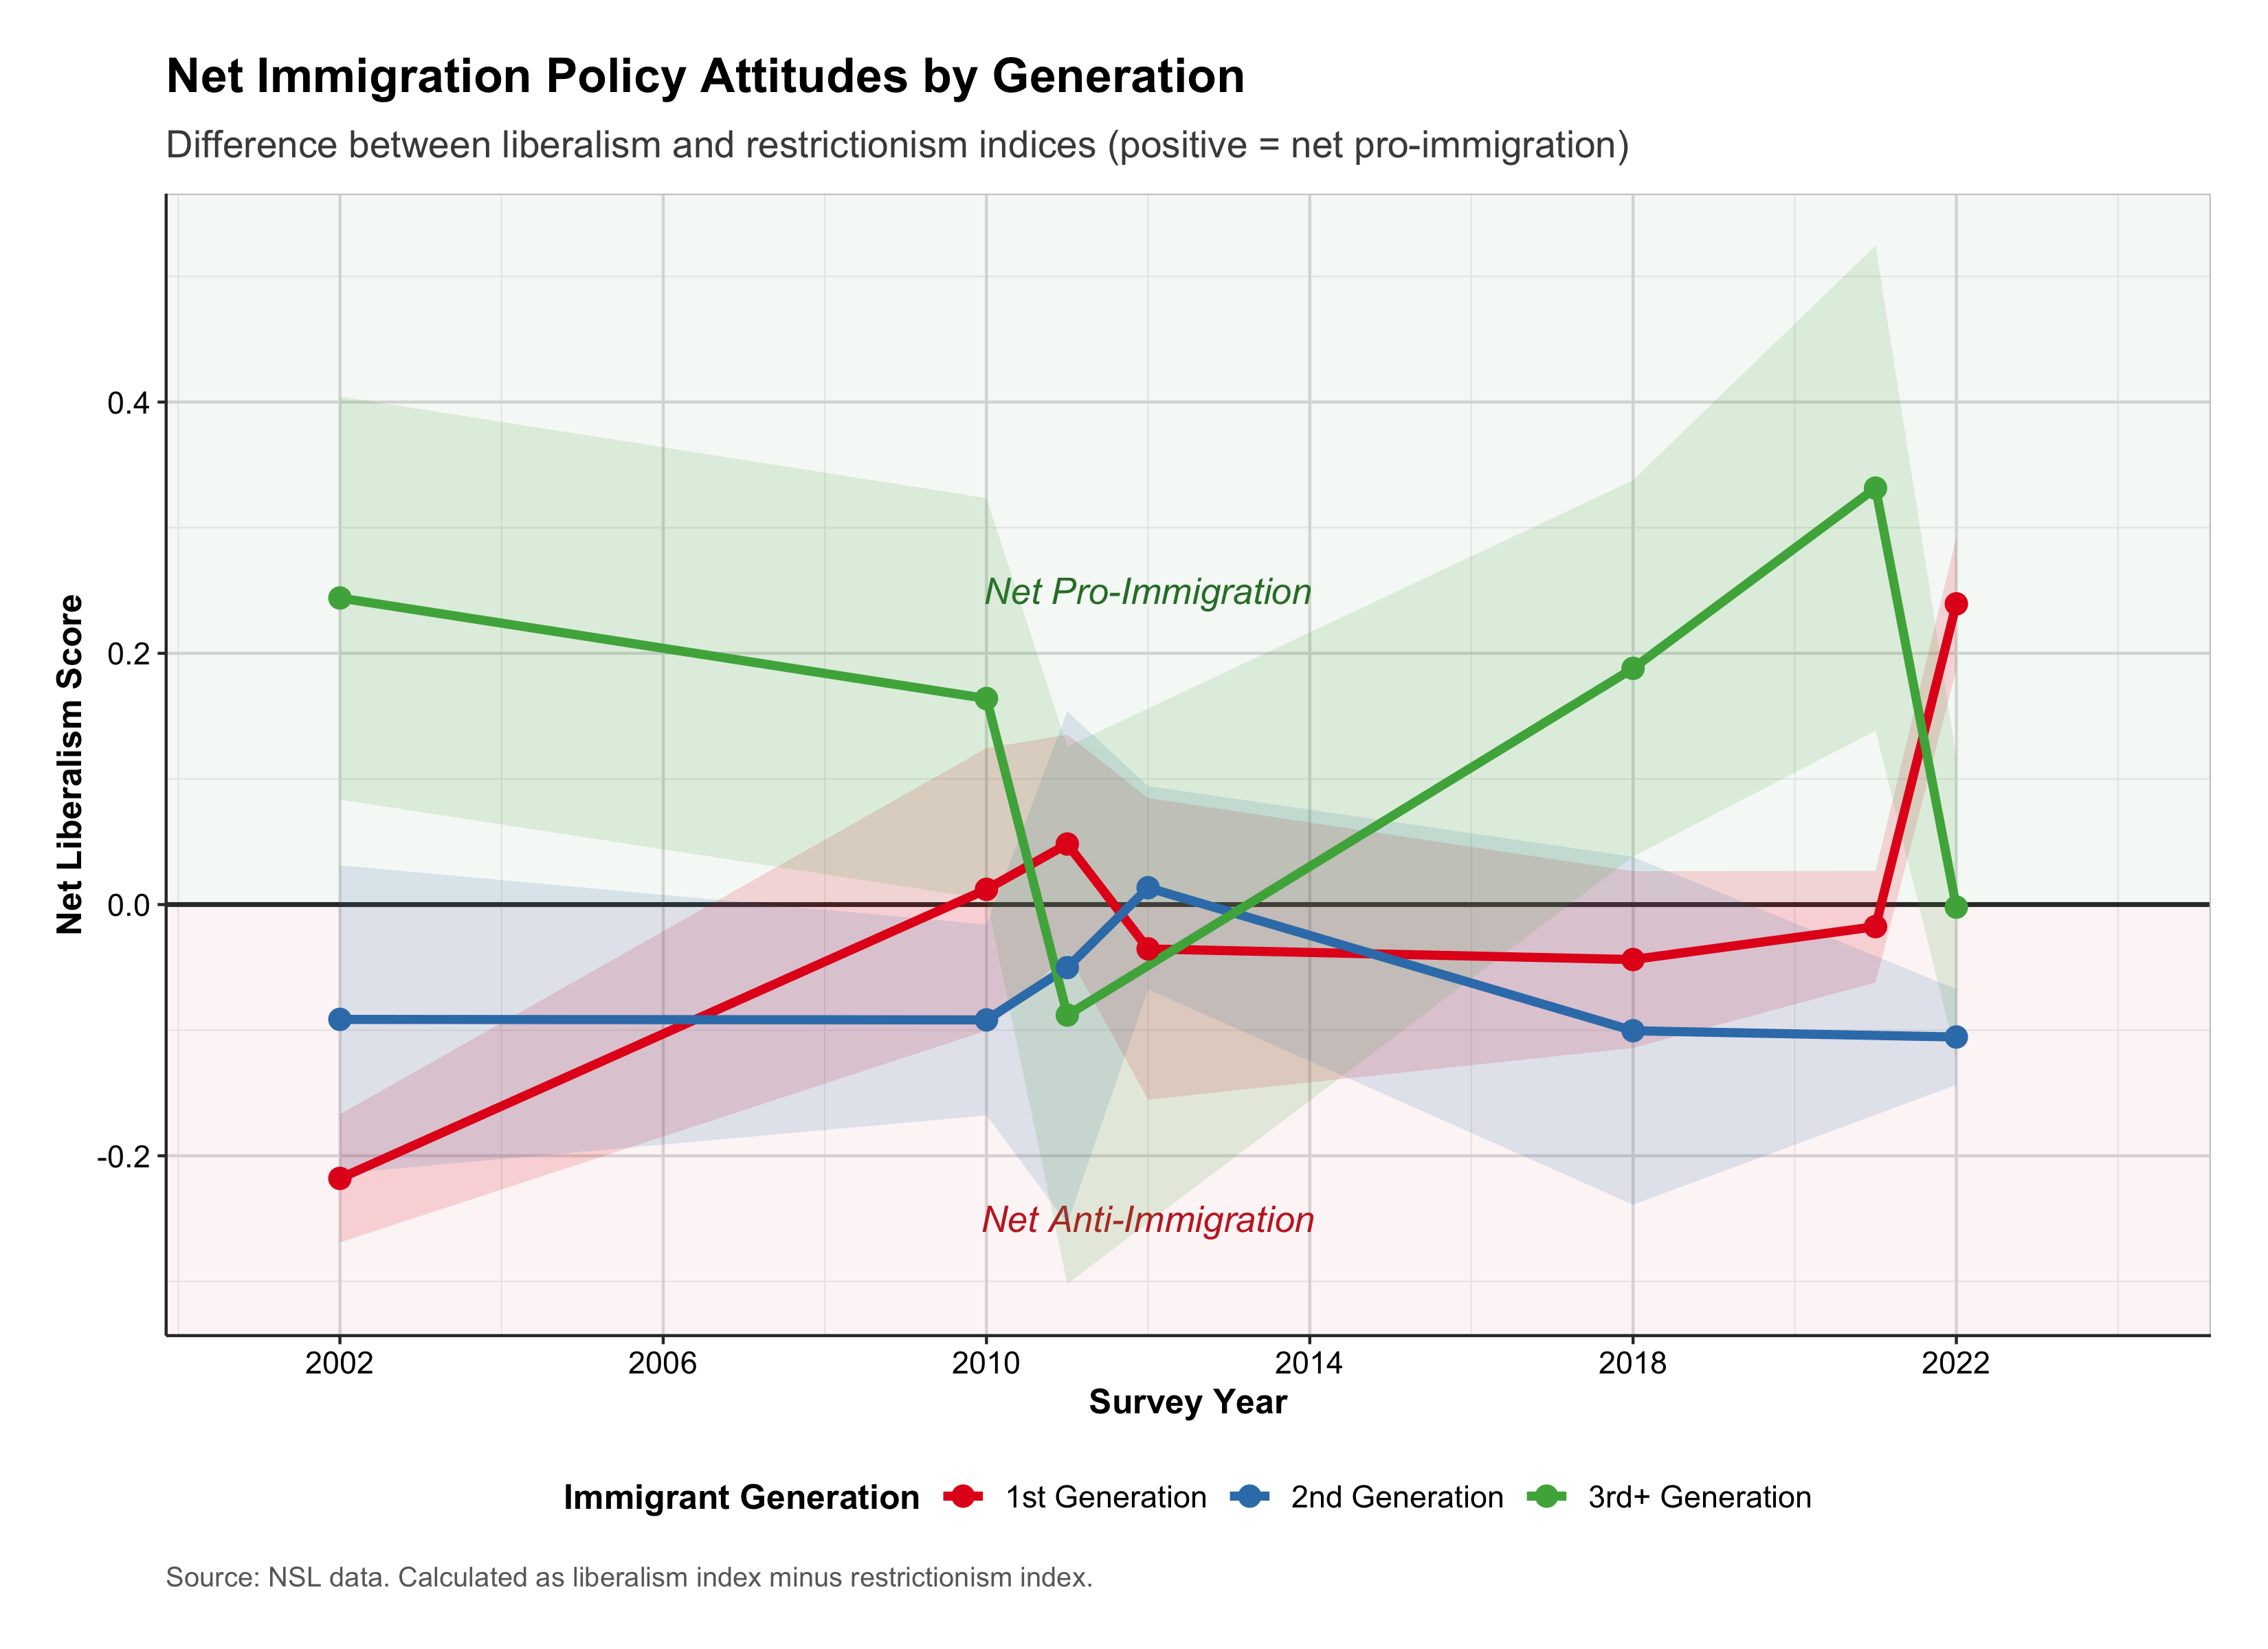
\includegraphics[width=0.9\textwidth]{figure_v4_4_net_liberalism.png}
    \caption{Net Immigration Policy Attitudes by Generation}
    \label{fig:net_liberalism}
\end{figure}

\begin{figure}[H]
    \centering
    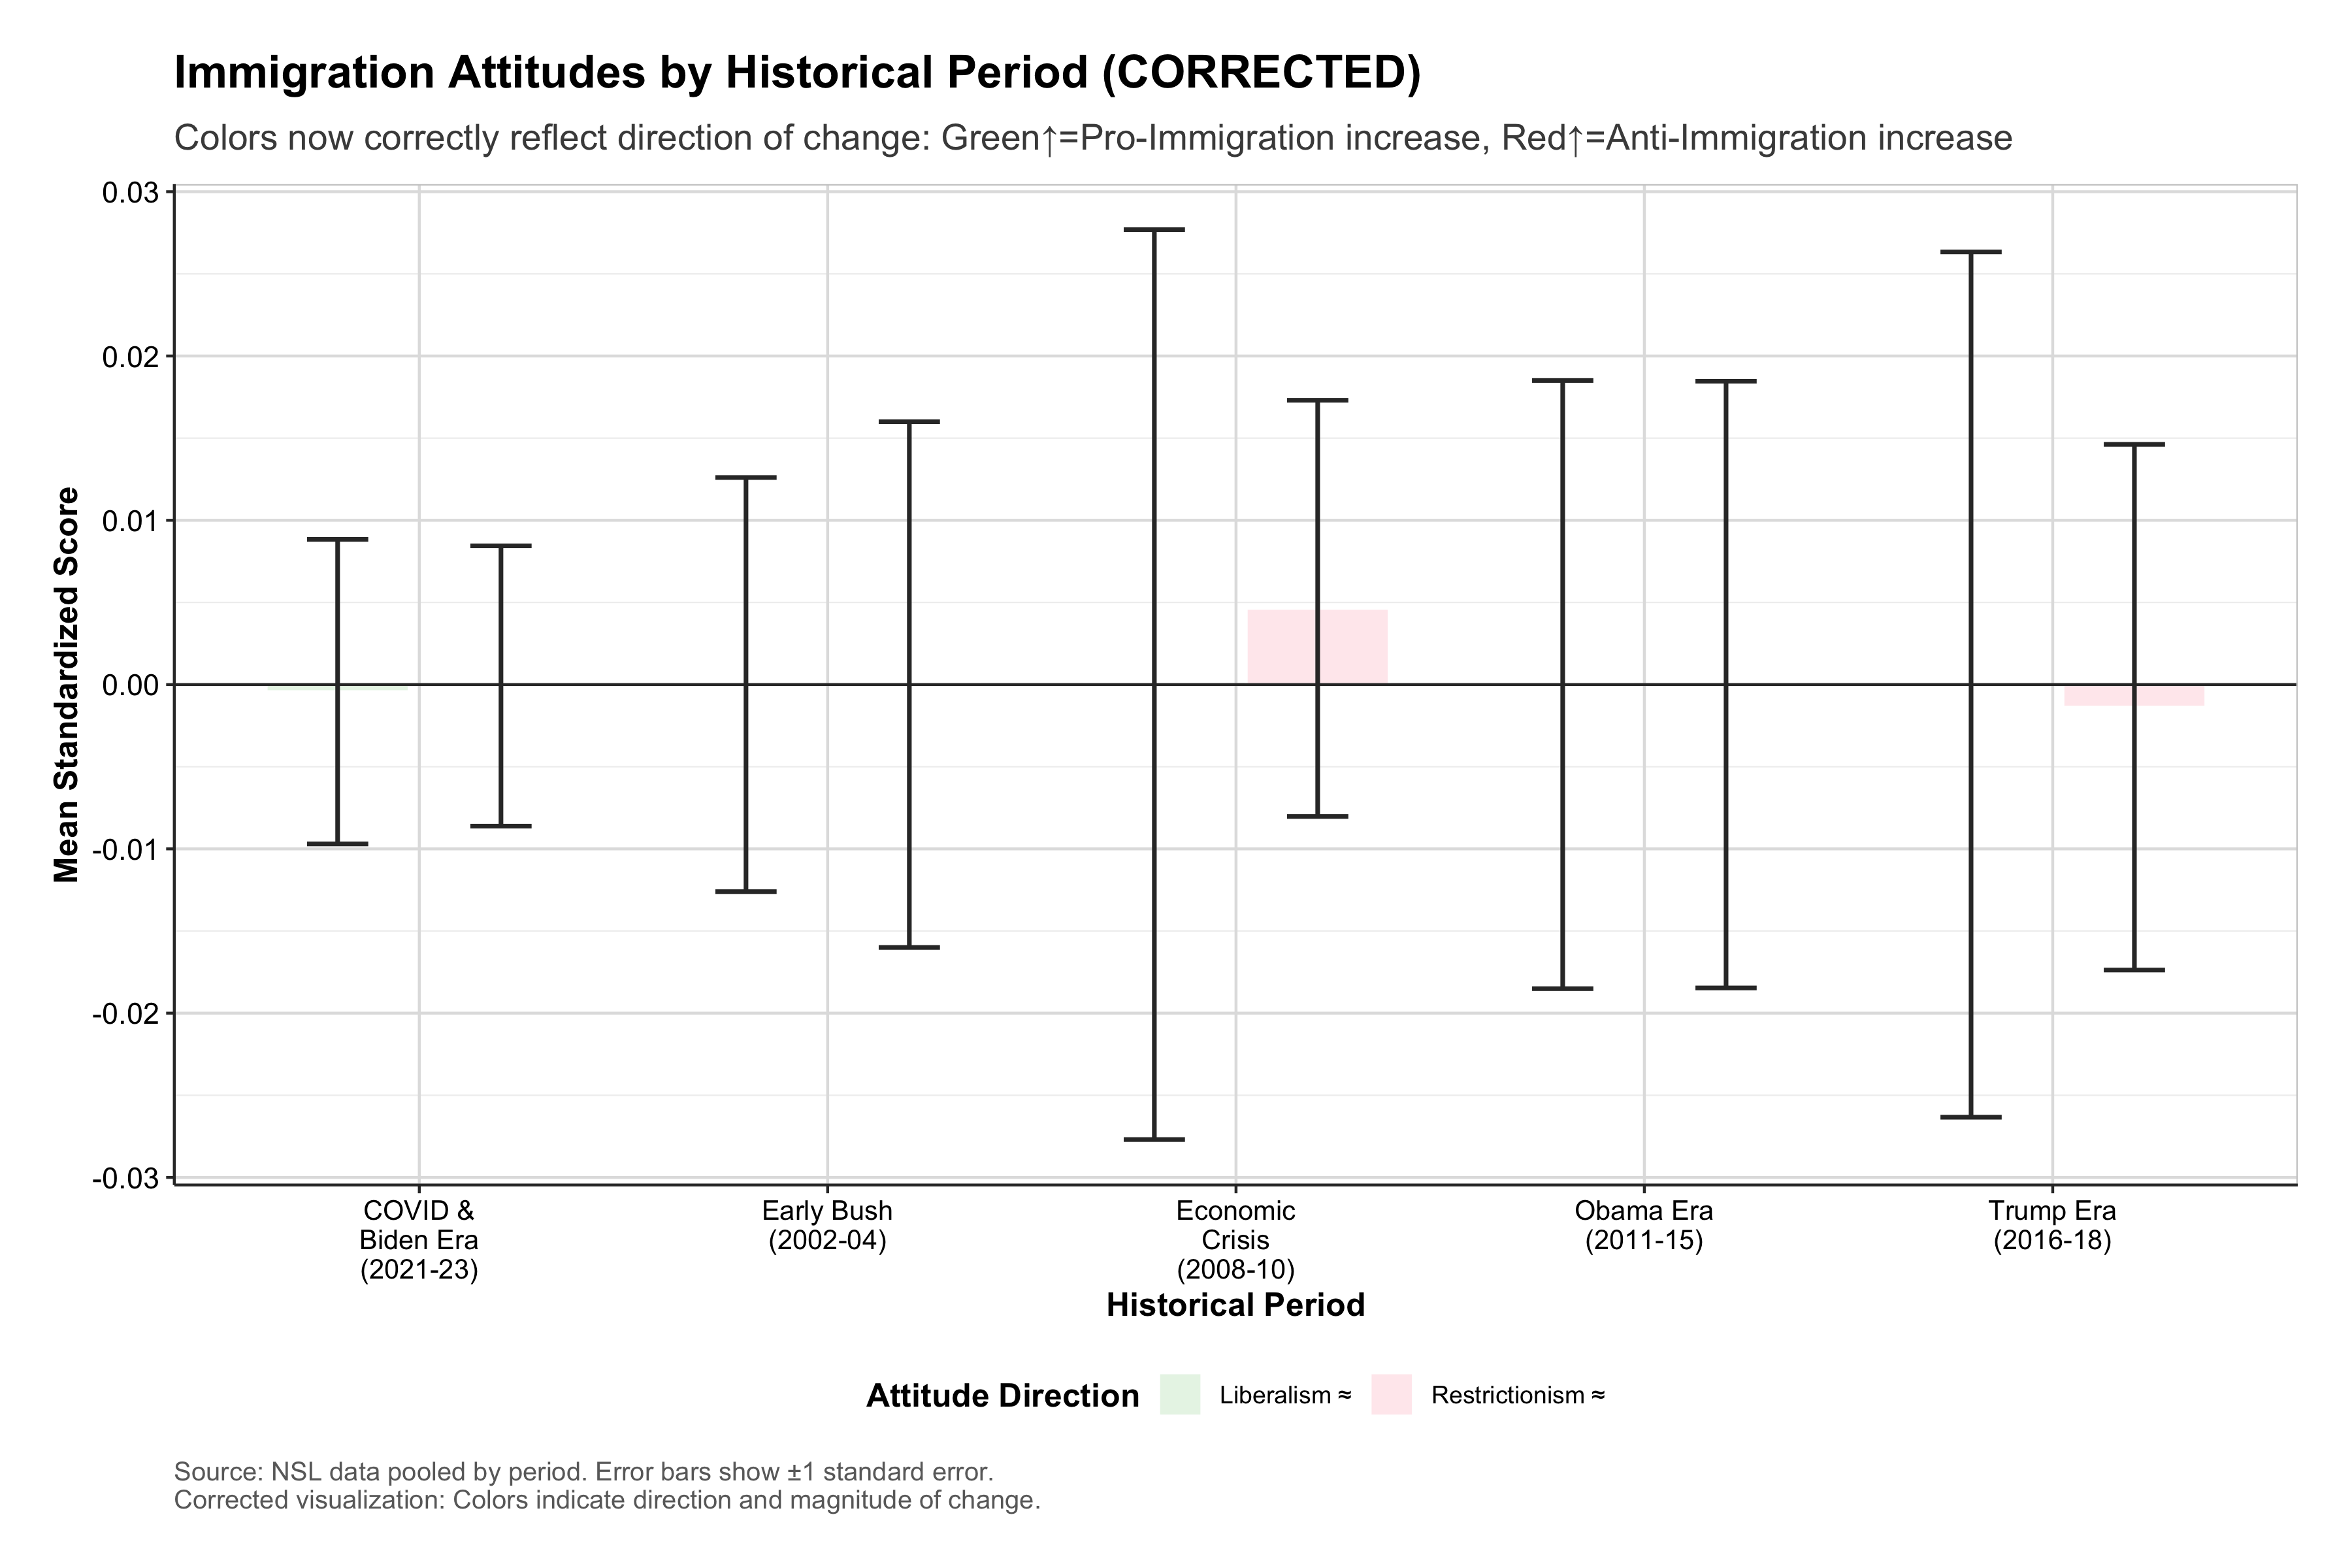
\includegraphics[width=0.9\textwidth]{figure_v4_4_period_effects_CORRECTED.png}
    \caption{Period Effects in Immigration Attitudes (Corrected Color Coding)}
    \label{fig:period_effects}
\end{figure}

\section{Central Argument: The Paradox Isn't a Paradox}

The phenomenon of ``immigrants against immigrants'' is \textbf{not} just hypocrisy or false consciousness. It may be the \textbf{logical outcome of political assimilation} into a polarized American society. As generations integrate, they adopt the nation's often contradictory political divisions.

\subsection{Mechanisms}
\begin{itemize}
    \item \textbf{Identity Signaling:} ``We are different from new immigrants''
    \item \textbf{Resource Competition:} Economic/social resource concerns
    \item \textbf{Assimilation Pressure:} Proving American belonging
    \item \textbf{Political Integration:} Adoption of American political divisions
\end{itemize}

\subsection{Disentangling Immigration Attitude}

\textbf{Immigration attitudes are genuinely multidimensional:}
\begin{itemize}
    \item Liberalism and restrictionism can coexist in one person!
    \item Attitudes are fragmented
    \item Different enforcement measures elicit different responses
\end{itemize}

\section{Theoretical \& Political Implications}

\subsection{Assimilation Theory Implications}

\textbf{Classical Assimilation: Partial Support}
\begin{itemize}
    \item 3rd+ generation most ``American'' in attitudes
    \item But process isn't linear across all dimensions
\end{itemize}

\textbf{Segmented Assimilation: Strong Support}
\begin{itemize}
    \item Multiple pathways evident across generations
    \item 2nd generation shows highest variance and complexity
\end{itemize}

\textbf{Reactive Ethnicity: Confirmed}
\begin{itemize}
    \item 1st generation mobilizes during threat periods
    \item Defensive response to Trump-era rhetoric
    \item Context-dependent attitude shifts
\end{itemize}

\subsection{Political and Policy Implications}

\textbf{For Theory:} Simple assimilation models are inadequate. ``Segmented assimilation'' (different pathways for different groups) and ``reactive ethnicity'' (mobilizing in response to threat) are better explanations.

\textbf{For Politics:} The ``Latino vote'' is not a monolith. Political messaging must be segmented by generation to be effective. Generational replacement will continue to shift the baseline of Hispanic political attitudes.

\textbf{For Policy:} Support for enforcement does not equal being ``anti-immigrant.'' Many individuals hold coexisting humanitarian and security concerns.

\subsection{The ``Immigrants Against Immigrants'' Phenomenon}

\subsubsection{Not a Paradox: A Logical Outcome}

\textbf{Integration Process:}
\begin{itemize}
    \item Integration $\rightarrow$ Adoption of American political divisions
    \item Generational distancing from immigrant identity
    \item Intragroup boundary-making processes
\end{itemize}

\textbf{Mechanisms:}
\begin{itemize}
    \item \textbf{Identity:} ``We are different from new immigrants''
    \item \textbf{Competition:} Economic/social resource concerns
    \item \textbf{Assimilation:} Proving American belonging
    \item \textbf{Context:} Period-specific political pressures (border wall discourse)
\end{itemize}

\section{Data Quality \& Methodological Strengths}

\subsection{Publication-Quality Standards}
\begin{itemize}
    \item \textbf{Temporal Coverage:} 21 years across 4 presidential administrations
    \item \textbf{Sample Size:} 37,496+ observations with generation recovery enhancement
    \item \textbf{Representative Sampling:} Pew Research Center's rigorous methodology
    \item \textbf{Survey Weights:} Population-representative estimates for 71\% of data
    \item \textbf{Missing Data Analysis:} Comprehensive assessment (59.12\% overall missing, within normal range)
    \item \textbf{Statistical Rigor:} Robust standard errors, sensitivity analysis
\end{itemize}

\subsection{Generation Recovery Enhancement (v3.1)}
\begin{itemize}
    \item \textbf{Problem:} Years 2008, 2009, 2015, 2018 had 0\% generation coverage
    \item \textbf{Solution:} Variable mapping correction recovered $\sim$6,200 observations
    \item \textbf{Impact:} Increased generation coverage from 60\% to 75\%+
    \item \textbf{Result:} Enhanced statistical power and temporal representation
\end{itemize}

\section{Conclusion: A Story of Political Incorporation}

\subsection{Central Finding}

``Immigrants against immigrants'' reflects \textbf{successful political assimilation}, not betrayal or false consciousness. It reveals how group boundaries shift across generations as populations integrate into polarized American political landscape.

\subsection{Methodological Lesson}
\begin{itemize}
    \item \textbf{Aggregation obscures reality} -- single indices hide crucial variation
    \item \textbf{Fragmented attitudes require nuanced measurement}
    \item \textbf{Temporal analysis essential} for immigration scholarship
    \item \textbf{Survey weights critical} for representative population-level findings
\end{itemize}

\subsection{Broader Implications}
\begin{enumerate}
    \item \textbf{Political incorporation involves adopting societal divisions}
    \item \textbf{Generational replacement will continue shifting baseline attitudes}
    \item \textbf{Immigration attitudes contain multiple, distinct dimensions}
    \item \textbf{Support exists for both humanitarian AND enforcement approaches}
\end{enumerate}

\subsection{Future Research Directions}
\begin{enumerate}
    \item \textbf{Qualitative follow-up:} Understanding mechanisms behind border wall attitudes
    \item \textbf{Experimental studies:} Testing framing effects on different measures
    \item \textbf{Regional analysis:} Geographic variation in generational patterns
    \item \textbf{Comparative perspective:} Including non-Hispanic populations
\end{enumerate}

\section{Technical Appendix}

\subsection{Key Statistical Results (v2.8 Survey-Weighted)}

\textbf{First Generation:}
\begin{itemize}
    \item Liberalism: +0.019 per year (p=0.021*)
    \item Restrictionism: +0.011 per year (p=0.004**)
\end{itemize}

\textbf{Second Generation:}
\begin{itemize}
    \item Liberalism: -0.005 per year (p=0.488, ns)
    \item Restrictionism: -0.015 per year (p=0.056, ns)
\end{itemize}

\textbf{Third+ Generation:}
\begin{itemize}
    \item Liberalism: -0.016 per year (p=0.158, ns)
    \item Restrictionism: -0.002 per year (p=0.908, ns)
\end{itemize}

\subsection{Available Visualizations}
\begin{itemize}
    \item \textbf{Main Trends:} \texttt{figure\_v4\_4\_main\_generation\_trends.png}
    \item \textbf{Disaggregated Components:} \texttt{figure\_v4\_4\_disaggregated\_components.png}
    \item \textbf{Net Attitudes:} \texttt{figure\_v4\_4\_net\_liberalism.png}
    \item \textbf{Generation Gap:} \texttt{figure\_v4\_4\_generation\_gap.png}
    \item \textbf{Period Effects:} \texttt{figure\_v4\_4\_period\_effects.png}
    \item \textbf{Two Dimensions:} \texttt{figure\_v4\_2\_dimensions\_scatter\_robust.png}
\end{itemize}

\subsection{Analysis Scripts}
\begin{itemize}
    \item \textbf{Core Analysis:} \texttt{IMMIGRATION\_ATTITUDES\_ANALYSIS\_v2\_8\_WEIGHTS\_CONTROLS\_SIMPLIFIED.R}
    \item \textbf{Generation Recovery:} \texttt{IMMIGRATION\_ATTITUDES\_ANALYSIS\_v3\_1\_GENERATION\_RECOVERY.R}
    \item \textbf{Disaggregated Analysis:} \texttt{DISAGGREGATED\_ANALYSIS\_v4\_3\_COMPONENTS.R}
    \item \textbf{Publication Visualizations:} \texttt{PUBLICATION\_QUALITY\_VISUALIZATIONS\_v4\_4.R}
\end{itemize}

\vspace{1em}
\noindent\rule{\textwidth}{0.4pt}

\begin{center}
\textbf{Analysis Version:} v2.8 (Survey-weighted) + v3.1 (Generation recovery) + v4.4 (Publication visualizations)\\
\textbf{Status:} Publication-ready\\
\textbf{Date:} August 2025
\end{center}

\end{document}
